\section{Planlægning}
Der blev fra projektets start udarbejdet en tidsplan.
Gennem forløbet har der sideløbende været fokus på både udvikling og rapport / dokumentations skrivning.
Gruppen ønskede ikke at lave enten udvikling eller rapport. Så samtidig med at man udviklede en del af systemet, skulle man også dokumentere denne del i den tilhørende dokumentation og samtidig skrive rapport afsnittet til samme område. \\
Dette har gjort at alt dokumentation er skrevet mens man havde det i frisk erindring.
Projektet har derfor haft nogle milepæle, som man skulle overholde for ikke at bruge for lang tid på dokumenterne samt udvikling. Disse kan ses på figur \ref{fig:Tidsplan}

\begin{figure} [H]
	\begin{center}
		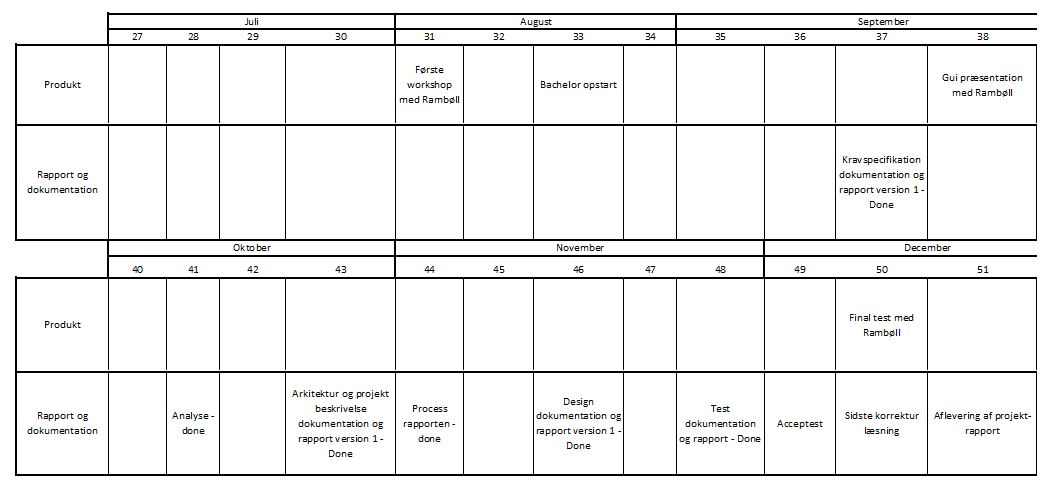
\includegraphics[height=10cm, width=18cm]{Moeder/Tidsplan}
	\end{center}
	\caption{Tidsplan for projektet}
	\label{fig:Tidsplan}
\end{figure}


